\chapter{WS16-17}\label{ch:klausurws16-17}

\section{Aufgabe 1}
\subsection{Lösungshinweis}

Die erste Aufgabe verdeutlicht, was bei einem \code{notifyAll()} und unsauber gesetzten Wartebedingungen passieren kann.\\
Sei folgender Quellcode gegeben:


\begin{minted}[mathescape,
    linenos,
    numbersep=5pt,
    gobble=2,
    fontsize=\small,
    frame=lines,
    framesep=2mm]{java}
    class Cond1AndCond2 {

        private boolean cond1;
        private boolean cond2;

        public synchronized void setCond1(boolean c) {
            cond1 = c;
            notifyAll();
        }

        public synchronized void setCond2(boolean c) {
            cond2 = c;
            notifyAll();
        }

        public synchronized void cond1AndCond2() {
            while(!cond1) {
                try {
                    wait();
                } catch(InterruptedException e) { }
            }

            while(!cond2) {
                try {
                    wait();
                } catch(InterruptedException e) {}
            }
            System.out.println("cond1 and cond2:" + cond1 + " " + cond2);
        }
    }
\end{minted}\\

Man sollte auf den ersten Blick meinen, dass \code{cond1} und \code{cond2} beide \code{true} sein müssen, damit die Ausgabe erfolgt.\\
Tatsächlich ist es aber so, dass es in der Methode zwei unterschiedliche Wartebedingungen gibt.\\
Die erste Wartebedingung schickt einen Thread in die Warteschlange, wenn \code{cond1 == false} gilt.\\
Setzt ein anderer Thread über \code{setCond1(true)} das Attribut entsprechend auf \code{true}, bewirkt der nachfolgende Aufruf von \code{notifyAll()}, dass alle \textit{wartenden} Threads aus der Warteschlange entfernt werden und erneut um eine Sperre des Objektes konkurrieren.\\
Erhält ein entsprechender Thread $t_w$ die Sperre auf das Objekt und kann seine \textit{while-wait-Schleife} verlassen, kann es vorkommen, dass er erneut in die Warteschlange eingereiht wird, wegen der nachfolgenden Wartebedingung \code{cond2 == false}.\\
Angenommen, ein weiterer Thread ruft nun \code{setCond2(true)} auf, und $t_w$ kommt aus der Warteschlange und konkurriert erneut und um die Sperre des Objektes, dann kann es vorkommen, das ein anderer Thread zunächst die Sperre erhält, \code{cond1} wieder auf \code{false} setzt, dann erhält $t_w$ die Sperre, überprüft die Wartebedingung \code{cond2 == false}.\\
Wegen \code{cond2} gelangt er aus der \textit{while-wait-Schleife} und die Ausgabe erfolgt - da zwischenzeitlich \code{cond1} wieder auf \code{false} gesetzt wurde, ist die erwartete Ausgabe nicht \code{true true}, sondern \code{false true} (s. Abbildung \ref{fig:cond1cond2}).\\

\begin{figure}
    \centering
    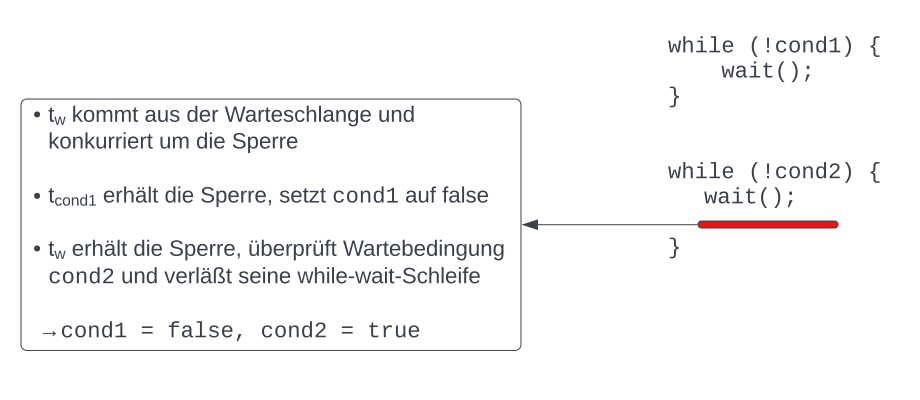
\includegraphics[scale=0.4]{chapters/Anhang/Klausuren/img/cond1cond2}
    \caption{in den rot markierten Bereich konkurriert $t_w$ um die Sperre des Objektes - wenn durch einen anderen Thread, der vor $t_w$ die Sperre erhält, \textit{cond1} auf \textit{false} gesetzt wird, stimmt die Ausgabe nicht mit der erwarteten überein. (Quelle: eigene)}
    \label{fig:cond1cond2}
\end{figure}

\noindent
Die korrekte Wartebedingung sollte lauten:

\begin{minted}[mathescape,
    linenos,
    numbersep=5pt,
    gobble=2,
    fontsize=\small,
    frame=lines,
    framesep=2mm]{java}
    public synchronized void cond1AndCond2() {
        while(!cond1 || !cond2) {
            try {
                wait();
            } catch(InterruptedException e) { }
        }
        System.out.println("cond1 and cond2:" + cond1 + " " + cond2);
    }
\end{minted}\\

Darüber hinaus müßte \code{notifyAll()} nur aufgerufen werden, wenn sowohl \code{cond1} als auch \code{cond2} auf \code{true} gesetzt sind, was leicht in den entsprechenden Methoden überprüft werden kann.